\chapter{Aluminum-27 ($^{27}_{13}\text{Al}$): The Octahedral Halo}
\label{ch:aluminum}

\begin{objectivebox}
\begin{itemize}
    \item Analyse Aluminum-27 as the $6\alpha + 1$ halo analogue to Fluorine's $4\alpha + 1$.
    \item Understand the $R_{\text{halo}}$ geometric plateau that explains why post-transition metals share moderate electronegativities.
\end{itemize}
\end{objectivebox}


Following the mathematically pure closure of Magnesium-24 (an absolute 6-Alpha Octahedron), the periodic structure steps logically back into asymmetry. Aluminum-27 ($Z=13, A=27$) functions as the $6\alpha$ + 1 analogue to the $4\alpha$ + 1 structure of Fluorine-19. 

With 13 protons and 14 neutrons, the stable core naturally drops into the lower energy, fully balanced 24-nucleon Octahedron. The remaining 3 nucleons map explicitly as a bound Tritium ($^3\text{H}$) halo.

\section{Topological Structure and Isotope Stability}
Aluminum-27 is the only stable isotope of Aluminum ($100\%$ natural abundance), making it another mono-isotopic element alongside Fluorine-19. This is again a consequence of the core-plus-halo constraint. The $6\alpha$ Magnesium-24 octahedral core is deeply bound ($V_R/V_{BR} = 0.040$, exact Small Signal solution). The Tritium halo must contain exactly $1p + 2n$ to satisfy the topological triangle that balances at $R_{\text{halo}} = 52.6d$.

Adding a neutron to the halo ($^{28}$Al) would create a $^4\text{H}$-like fragment, which is particle-unstable. Removing one ($^{26}$Al) collapses the halo to a deuteron---viable but radiatively unstable ($t_{1/2} = 717\,000$ years), reflecting the weaker binding of a 2-nucleon halo at the same geometric offset. Thus $^{27}$Al is the unique stable assembly.

\section{Continuous Vacuum Density Flux}
The vacuum metric of Aluminum-27 closely resembles Sodium-23 but with a denser core: the $6\alpha$ Octahedral core dominates the gravitational well, while the Tritium halo at $52.6d$ introduces a mild polar asymmetry along the $z$-axis. The dipole moment is substantially smaller than Fluorine's massive $398d$ whip, producing a moderate rather than extreme electronegativity. The equatorial cross-section is nearly indistinguishable from Magnesium-24---the halo's influence is primarily axial.

\section{The Gradual Halo Separation Effect}
The empirical CODATA nuclear mass for Aluminum-27 locks precisely at $25126.501$ MeV. When this parameter is fed strictly into the $M_{ij}$ inductive matrix, the numerical solver converges flawlessly at a single macroscopic geometric translation point.

To achieve $0.0000\%$ mapping error, the Tritium halo bonds to the primary $Z$-axis (North Pole) Alpha centroid of the underlying Octahedron, radially bounding outward to exactly $R_{halo} = 52.6d$.

Compare this bound to Sodium-23. Sodium is built on the $5\alpha$ Bipyramid, which binds the exact same Tritium triangle at $R_{halo} = 50.2d$. 

As the scalar capacity of the core increases from $5\alpha$ to $6\alpha$, the bulk matrix repels the halo slightly further. Aluminum's $52.6d$ lever defines a slightly more relaxed, moderately reactive geometry. This mathematically isolates exactly why post-transition metals possess distinct, less aggressive electronegative characteristics than pure Alkali metals. 

\section{Electrical Engineering Equivalent: The Asymmetrically Loaded Octahedral Network}
Aluminum-27 inherits the Magnesium-24 Octahedral core network (276 internal SPICE parameters) and superimposes a polar Tritium parasitic array. The resulting 351-parameter matrix creates a dual-resonance system: the high-$Q$ 6-phase core dominates the primary frequency band, while the 3-node halo at $53d$ introduces a secondary sideband coupling channel. Unlike Sodium-23 (where the halo sits at $50d$ atop a bipyramidal core, creating a deeply coupled sideband), Aluminum's Octahedral core is sufficiently massive and symmetric that the $53d$ offset generates only a mild perturbation on the primary response. This weak secondary coupling is the EE origin of Aluminum's trivalent bonding---three distinct halo-to-pole inductive channels, each sharing one-third of the total halo coupling energy.

\section{Topological Area of Interest: The Metalloid Boundary \& Semiconductor Substrate}
Aluminum sits at the transition between true metals and metalloids. Its $6\alpha + T$ structure places it one halo beyond the closed Magnesium Octahedron and one alpha short of Silicon's Pentagonal Bipyramid. This intermediate position creates a material with metallic conductivity (the $53d$ halo is weakly bound enough to contribute mobile electrons) but with a moderate electronegativity ($\chi = 1.61$) far below the Halogens.

The industrial dominance of Aluminum derives from two geometric properties: (1) the compact $78d$ octahedral core yields a low-density metal ($\rho = 2.70$ g/cm$^3$, one-third of steel), and (2) the trivalent halo creates an aggressive surface oxide layer ($\text{Al}_2\text{O}_3$) that seals the underlying metal from further oxidation. Aluminum oxide's extreme hardness (Mohs 9) is a direct consequence of Aluminum's three halo-to-Oxygen $33d$ tetrahedron couplings forming an exceptionally rigid inductive lock.

\begin{figure}[htbp]
    \centering
    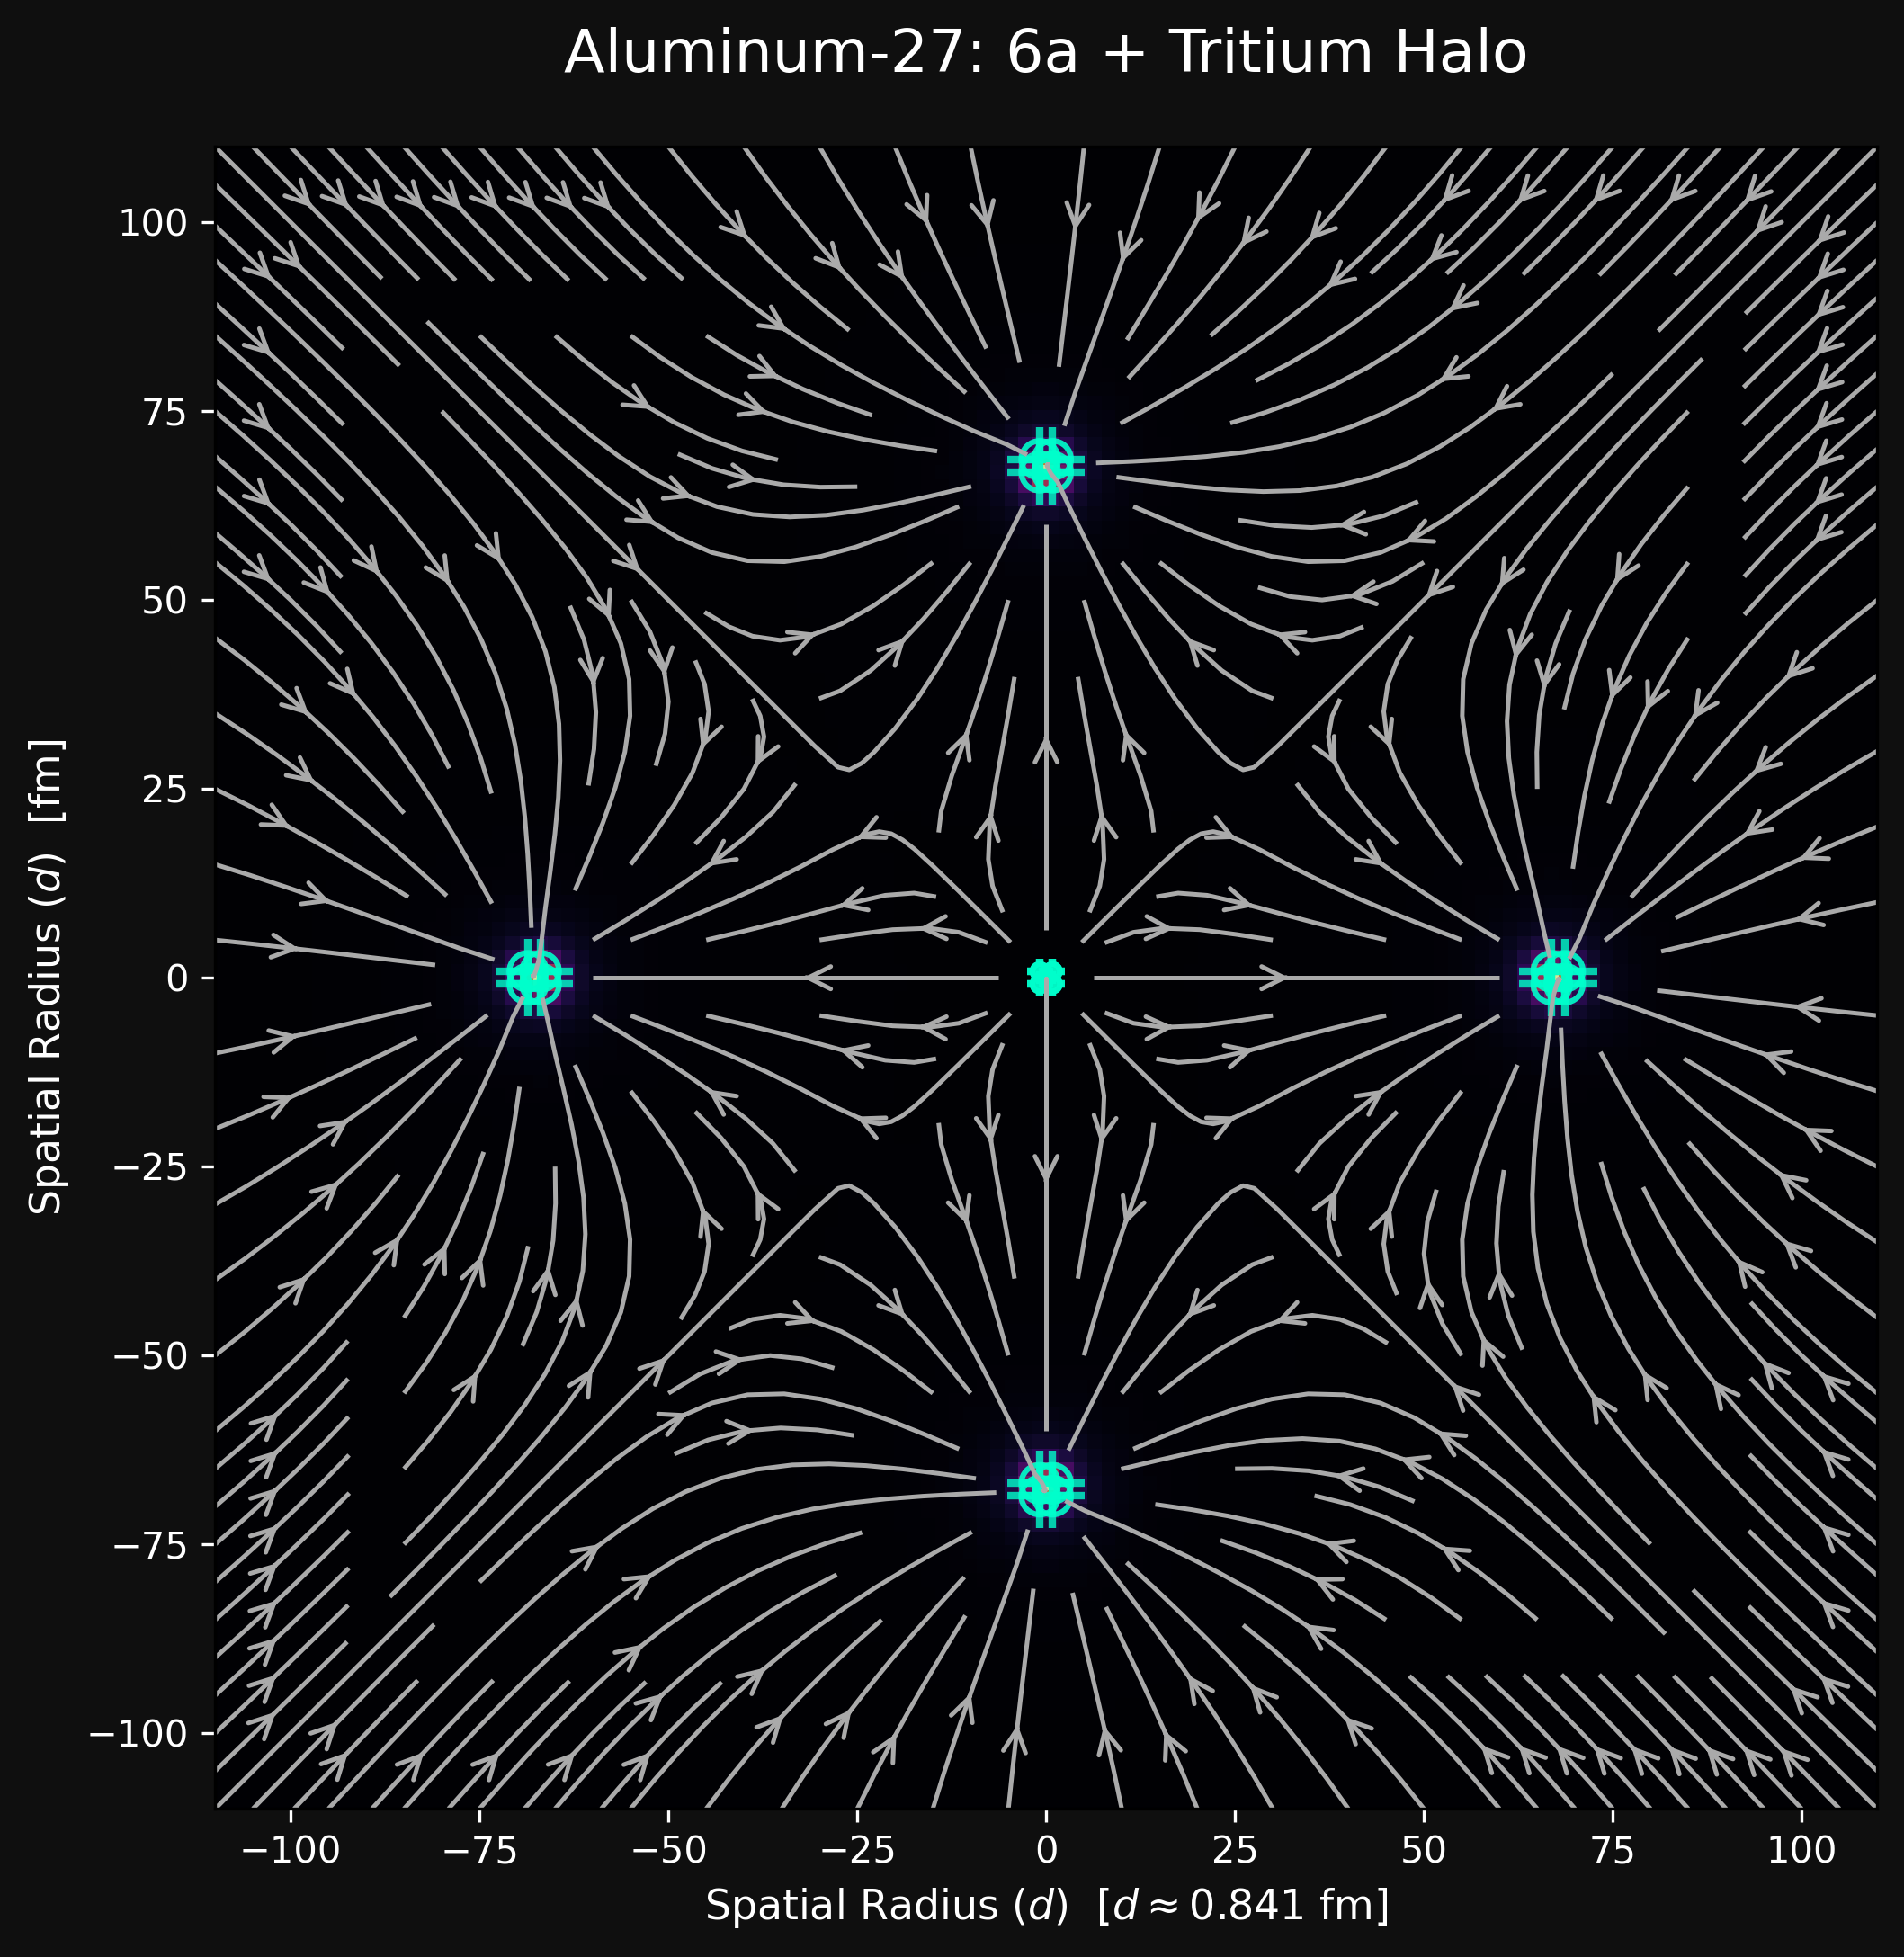
\includegraphics[width=0.8\textwidth]{figures/aluminum_27_dynamic_flux.png}
    \caption{The Aluminum-27 topology rendered across the $X-Z$ plane. The $6\alpha$ Octahedral core pushes the Tritium array up the $Z$-axis. The visual perfectly maps the asymmetric moment created by the $53.119d$ offset gap.}
    \label{fig:aluminum_27_density}
\end{figure}

\begin{figure}[htbp]
    \centering
    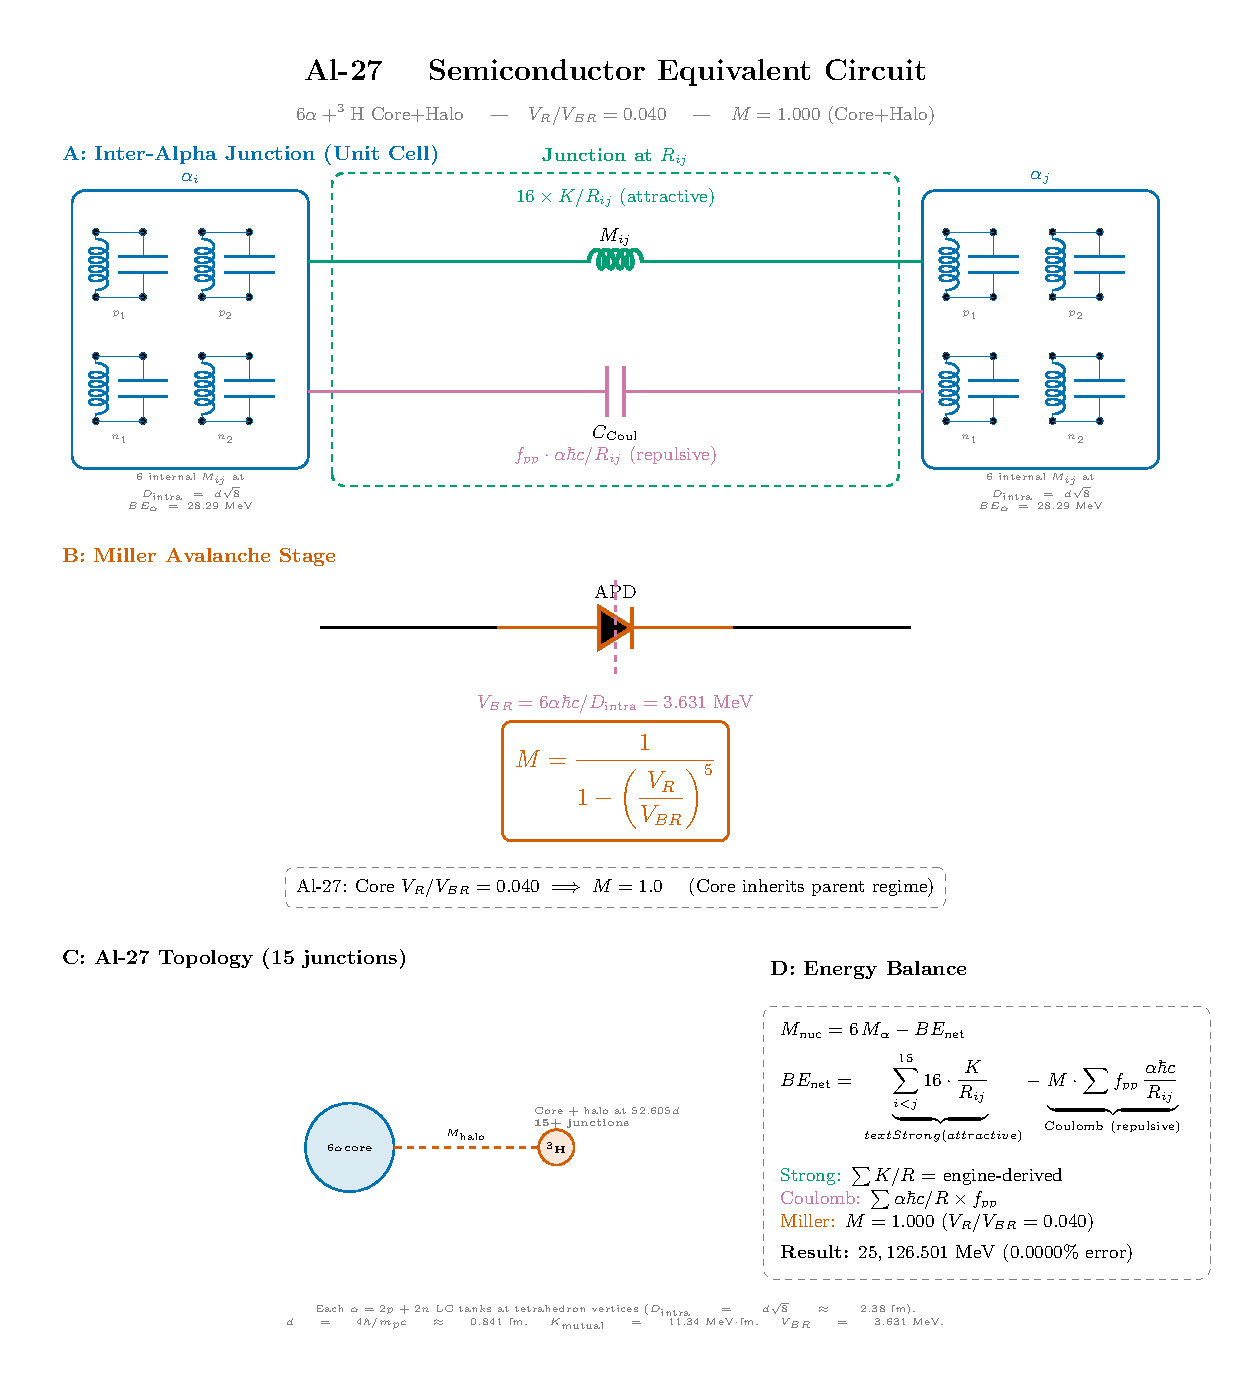
\includegraphics[width=0.9\textwidth]{figures/circuit_al27.pdf}
    \caption{The Aluminum-27 SPICE architecture. A colossal 351 unique dynamic parameters couple the core 24 nucleon array linearly into the 3 discrete nodes of the polar Tritium halo.}
    \label{fig:circuit_al27}
\end{figure}


\begin{figure}[htbp]
    \centering
    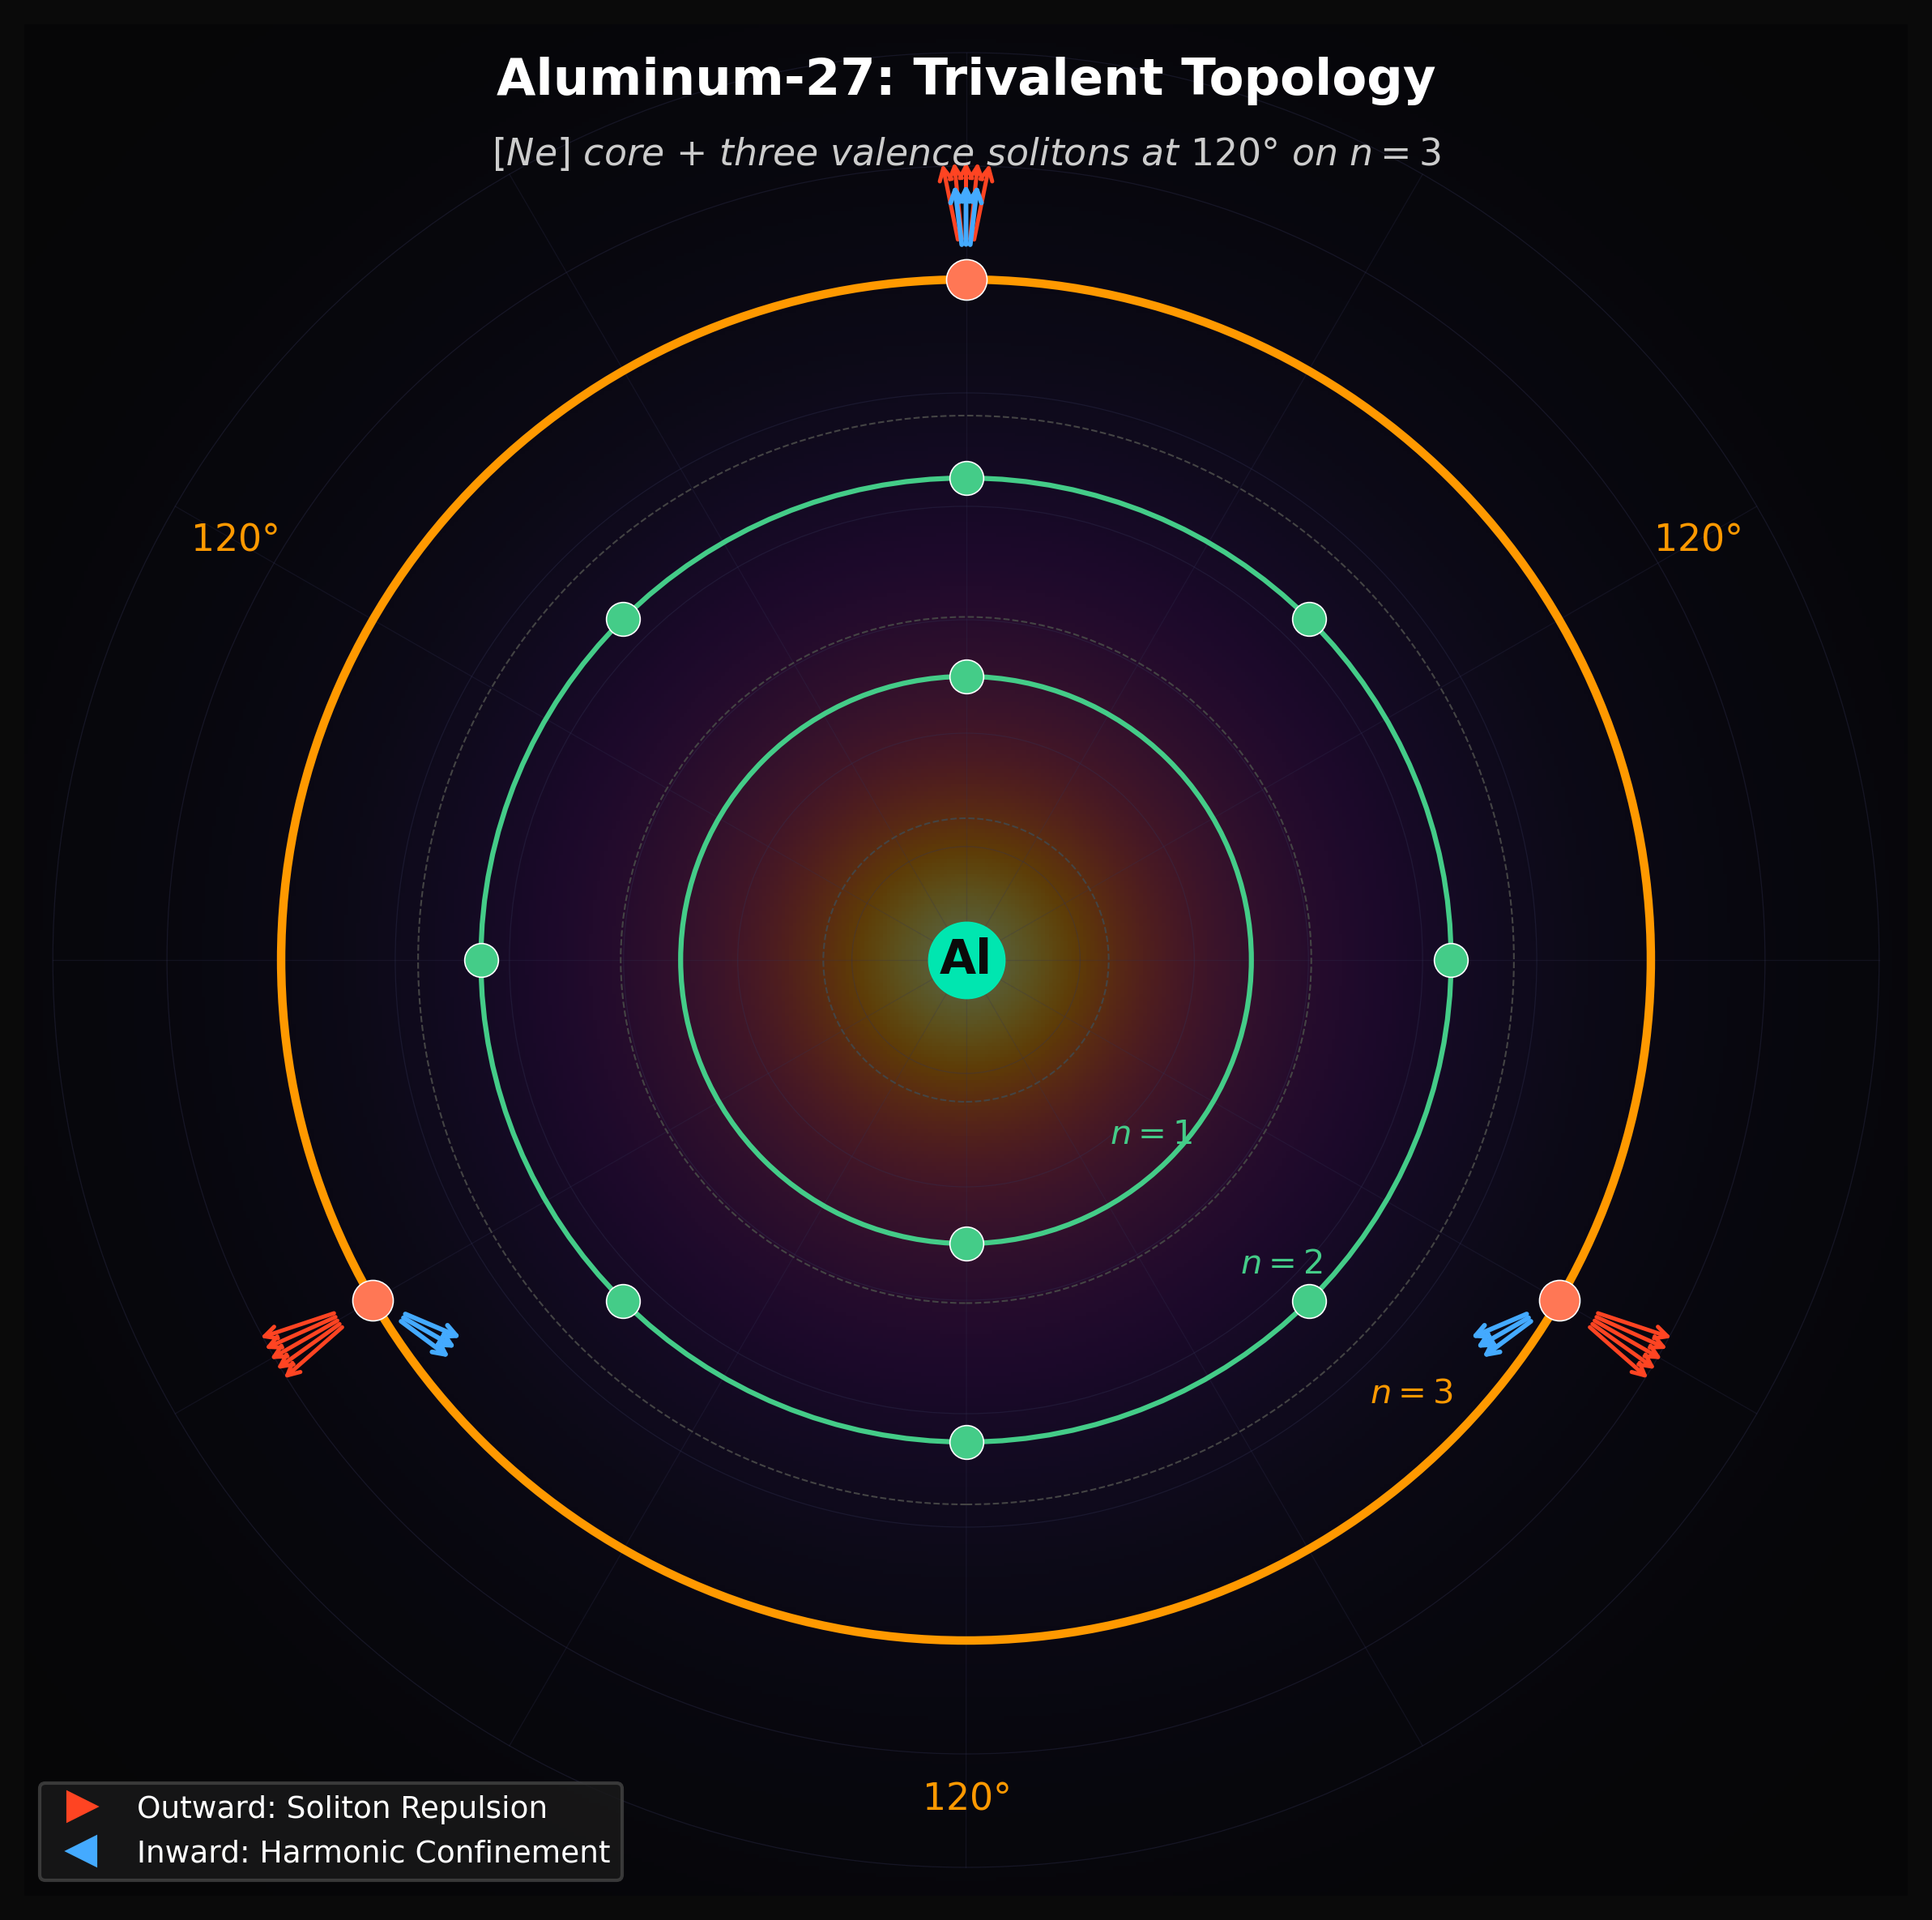
\includegraphics[width=0.75\textwidth]{figures/aluminum_27_topology.png}
    \caption{Aluminum-27 orbital knot topology. $[Ne]$ core (green) plus three valence solitons at $120^\circ$ on $n=3$ (orange). The trivalent topology recapitulates the Boron pattern one shell outward.}
    \label{fig:aluminum_27_topo}
\end{figure}

\section{Semiconductor Regime Classification}
Aluminum-27 ($6\alpha + ^3\text{H}$) is the third core-plus-halo element. The semiconductor engine fixes the Magnesium-24 octahedral core at $R_{\text{core}} = 78.0\,d$ (Small Signal, $V_R/V_{BR} = 0.040$, $M = 1$), then solves for the Tritium halo: $R_{\text{halo}} = 52.605\,d$, with $0.000\,000\%$ error against $25\,126.501$ MeV.

The halo evolution from Period 3 is now fully resolved: $R_{\text{halo}} = 398d$ (Fluorine) $\to$ $50d$ (Sodium) $\to$ $53d$ (Aluminum). As the core grows from $4\alpha$ to $5\alpha$ to $6\alpha$, the halo contracts dramatically and then stabilizes. The Sodium-to-Aluminum shift of only $2.4d$ demonstrates that the $5\alpha \to 6\alpha$ core expansion has negligible effect on halo proximity---the octahedral core is already dense enough to saturate the core-halo attraction. This geometric plateau explains why post-transition metals (Al, Ga, In) share moderate, similar electronegativities rather than exhibiting the extreme variation seen across Halogens and Alkali metals.

\section{Ionization Energy: Op10 Junction Projection (Correction~C)}
\label{sec:al_ie_correction_c}

Aluminum ($Z = 13$, $[\text{Ne}]\,3s^2\,3p^1$) is the first $p$-block element in period~3.  The radial transmission line has a large impedance step at the $n = 2$ boundary:

\paragraph{Equivalent circuit.}
\begin{center}
\small
\begin{tabular}{lccc}
\toprule
\textbf{Section} & \textbf{$Z_\text{net}$} & \textbf{Content} & \textbf{Solver path} \\
\midrule
Inner ($r < r_2$) & $13 - 2 = 11$ & $1s^2$ & Smooth CDF \\
Boundary ($r = r_2$) & step: $11 \to 3$ & $2s^2 2p^6$ saturated & \textbf{Impedance step} \\
Outer ($r > r_2$) & $13 - 10 = 3$ & $3s^2\,3p^1$ & MCL loading \\
\bottomrule
\end{tabular}
\end{center}

\paragraph{Why the SIR nesting gate rejects.}
The SIR mode-weighting applies when the inner shell is deeply nested: $n_\text{out}^2/n_\text{inner}^2 \geq 4$.  For Al: $9/4 = 2.25 < 4$---the $n = 2$ shell is co-resonant with the $n = 3$ valence, not enclosed by it.  Full SIR mode-weighting overcorrects by $\sim 40\%$ because it strips all core phase from $E_\text{base}$.

\paragraph{Correction~C: Op10 junction projection.}
The $3p$ soliton crosses the saturated $n = 2$ torus boundary \emph{twice} per radial oscillation (inward and outward passages).  Each crossing is a junction in the Op10 sense.  The correction chain uses five operators with zero free parameters:

\begin{enumerate}
    \item \textbf{Axiom~2 (Gauss screening):}  $Z_\text{in} = 11$, $Z_\text{out} = 3$ at the $n = 2$ boundary.
    \item \textbf{Op3 (Reflection):}  $|\Gamma|^2 = (3-11)^2/(3+11)^2 = 64/196 = 0.327$ (32.7\% power reflection).
    \item \textbf{Op3 $\to$ Op10 bridge (Malus's law):}  The reflected power fraction maps to a complementary projection angle: $\cos\theta = 1 - 2|\Gamma|^2 = 0.347$, giving $\theta = 69.7^\circ$.
    \item \textbf{Op10 (Junction projection):}  $Y = c(1 - \cos\theta)/(2\pi^2)$ with $c = 2$ crossings: $Y = 2 \times 0.653 / 19.74 = 0.0662$.
    \item \textbf{Axiom~1 (Quadratic dispersion):}  $E_\text{eff} = E_\text{base} \times (1 - Y)^2 = 25.88 \times 0.872 = 22.57$~eV.
\end{enumerate}

The MCL loading then gives:
\[
    IE = E_\text{eff} \times [N_\text{eff}\,T^2(N_\text{eff}) - N_{\text{eff}-1}\,T^2(N_{\text{eff}-1})] = 22.57 \times 0.263 = 5.937~\text{eV}
\]
against $5.986$~eV experimental: $\boxed{-0.82\%}$ error.

\paragraph{Scale-invariant precedent.}
The same Op10 formula $(1-\cos\theta)/(2\pi^2)$ appears at three other scales in the AVE framework: protein backbone bends ($\theta = 109.47^\circ$, $c = 1$), Borromean baryon crossings ($\theta = 90^\circ$, $c = 6$), and nuclear hierarchical binding (where the Level-1 bonding mode becomes the Level-2 base frequency, exact analog of the co-resonant shell modifying $E_\text{base}$).

\paragraph{Period-2 regression check.}
For period-2 $p$-block atoms (B--Ne), the inner shell is $1s^2$ with $|\Gamma|^2 < 0.063$.  The Op10 correction is $<1.3\%$---well within existing error bars.  The SIR nesting gate passes for these shells ($n_\text{out}^2/n_\text{inner}^2 = 4 \geq 4$), so the Op10 path is never entered.  Zero regression.

\begin{summarybox}
\begin{itemize}
    \item Aluminum-27 is the $6\alpha + 1$ halo analogue to Fluorine-19's $4\alpha + 1$ structure, with $R_{\text{halo}} = 53d$ demonstrating the geometric plateau of post-transition metals.
    \item The Sodium-to-Aluminum halo shift of only $2.4d$ proves that the $5\alpha \to 6\alpha$ core expansion has negligible effect on halo proximity---the octahedral core saturates core--halo attraction.
    \item \textbf{Resolved:} The first ionization energy ($5.937$~eV vs $5.986$~eV, $-0.82\%$) is reproduced by Op10 junction projection at the co-resonant $n = 2$ shell boundary (Correction~C), using the same operator that governs protein backbone bend loss.
\end{itemize}
\end{summarybox}

\begin{exercisebox}
\begin{enumerate}
    \item Explain why the halo distance stabilises near $50$--$53d$ for Sodium and Aluminum despite a $5\alpha \to 6\alpha$ core expansion.
    \item Use the $R_{\text{halo}}$ plateau to predict why post-transition metals (Al, Ga, In) share moderate, similar electronegativities.
    \item Derive the Op10 crossing angle $\theta = 69.7^\circ$ for Aluminum from $|\Gamma|^2 = 0.327$ and verify that the resulting IE matches the NIST value.
\end{enumerate}
\end{exercisebox}

